\documentclass[crop,tikz]{standalone}

\usepackage{tikz}
\usetikzlibrary{shapes.geometric}
\usetikzlibrary{patterns}
\usetikzlibrary{matrix}
\usetikzlibrary{fit}
\usetikzlibrary{decorations.pathreplacing}
\usetikzlibrary{calc,positioning,tikzmark,matrix.skeleton}

\pagenumbering{gobble}

\begin{document}

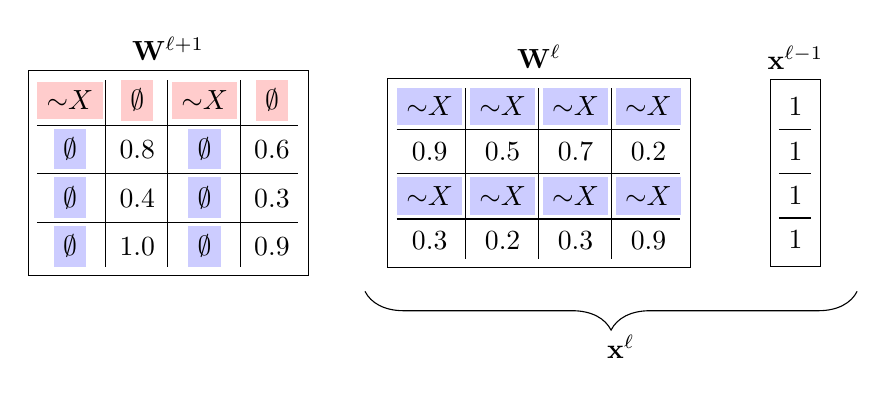
\begin{tikzpicture}[>=stealth]
    % Layer 2 matrix
    \matrix (W2) [
        matrix of math nodes, 
        %left delimiter={(},
        %right delimiter={)},
        style grid={draw, thin},
        label=above:\( \mathbf{W}^{\ell + 1} \),
        draw,
        sharp corners,
        column sep=1mm,
        row sep=1mm,
    ] {
        % 0.9 & 1.0 & 0.8 & 0.1 \\ % original values
        %|[fill=red!10]| \sim X & |[fill=red!10]| \sim X & |[fill=red!10]| \sim X & |[fill=red!10]| \sim X \\
        |[fill=red!20]| {\sim}X & |[fill=red!20]| \emptyset & |[fill=red!20]| {\sim}X & |[fill=red!20]| \emptyset \\
        |[fill=blue!20]| \emptyset & 0.8 & |[fill=blue!20]| \emptyset & 0.6 \\
        |[fill=blue!20]| \emptyset & 0.4 & |[fill=blue!20]| \emptyset & 0.3 \\
        |[fill=blue!20]| \emptyset & 1.0 & |[fill=blue!20]| \emptyset & 0.9 \\
    };
    
    % Layer 1 matrix
    \matrix (W1) [
        matrix of math nodes, 
        %left delimiter={(},
        %right delimiter={)},
        style grid={draw, thin},
        label=above:\( \mathbf{W}^{\ell} \),
        right=1cm of W2,
        draw,
        sharp corners,
        column sep=1mm,
        row sep=1mm,
    ] {
       % 0.2 & 0.4 & 0.2 & 0.6 \\
        |[fill=blue!20]| {\sim}X & |[fill=blue!20]| {\sim}X & |[fill=blue!20]| {\sim}X & |[fill=blue!20]| {\sim}X \\
        0.9 & 0.5 & 0.7 & 0.2 \\
        % 0.9 & 0.6 & 0.4 & 0.5 \\
        |[fill=blue!20]| {\sim}X & |[fill=blue!20]| {\sim}X & |[fill=blue!20]| {\sim}X & |[fill=blue!20]| {\sim}X \\
        0.3 & 0.2 & 0.3 & 0.9 \\
    };
    
    % Right-hand side vector
    \matrix(x0)[
        matrix of math nodes,
        %left delimiter={(},
        %right delimiter={)},
        style grid={draw, thin},
        label=above:\( \mathbf{x}^{\ell - 1} \),
        right=1cm of W1,
        draw,
        sharp corners,
        column sep=1mm,
        row sep=1mm,
    ] {
        1 \\
        1 \\
        1 \\
        1 \\
    };
    
    % Arrows
    \draw [decorate,decoration={brace,amplitude=14pt},rotate around={90:(0.5,0.5)},=0] (-1.5,-7.75) -- (-1.5,-1.5);
    \node[] at (5.75,-2.2) {$\mathbf{x}^{\ell}$};
\end{tikzpicture}

\end{document}